%%%%%%%%%%%%%%%%%%%%%%%%%%%%%%%%%%%%%%%%%%%%%%%%%%%%%%%%%%%%%%%%%%%%%%%%%%%%%
% Chapter 1: Introducción 
%%%%%%%%%%%%%%%%%%%%%%%%%%%%%%%%%%%%%%%%%%%%%%%%%%%%%%%%%%%%%%%%%%%%%%%%%%%%%%%

%---------------------------------------------------------------------------------
\section{¿Qué es SIMDE?}
\label{1:sec:1}

En el año dos mil cuatro, el por aquel entonces estudiante de esta universidad, 
Iván Castilla Rodríguez - y ahora tutor de este trabajo de fin de grado-, 
desarrolló como proyecto final de carrera un Simulador Didáctico para la enseñanza 
de arquitectura de computadores, bautizado como Simde. 

Este simulador permite al usuario representar de forma visual los dos grandes tipos 
de máquinas que implementan el paralelismo a nivel de instrucción (las máquinas 
Superescalares y las VLW). Y desde entonces se ha estado utilizando por los alumnos 
de las asignaturas relacionadas, tal como puede ser la asignatura de arquitectura de 
computadores, de la especialidad de Ingeniería de Computadores.

%---------------------------------------------------------------------------------
\section{Motivación para el trabajo}
\label{1:sec:2}

\begin{itemize}
  \item Item 1
  \item Item 2
  \item Item 3
\end{itemize}

%---------------------------------------------------------------------------------
\section{Breve introducción a los fundamentos teóricos}
\label{1:sec:3}

Bla, bla, bla

%---------------------------------------------------------------------------------
\begin{figure}[!th]
\begin{center}
\includegraphics[width=0.5\textwidth]{images/arbolbinario.eps}
\caption{Ejemplo}
\label{fig:ArbolBinario}
\end{center}
\end{figure}
%------------------------------------------------------------------------------

